\chapter{Ecossistemas Empreendedores e Sistemas Regionais de Inovação}
\tagAV{AV1 (30\%)}\ \tagTerritorio

\begin{capObjetivos}
Ao concluir este capítulo, você será capaz de:
\begin{itemize}[leftmargin=1.4em, itemsep=2pt]
  \item Distinguir a abordagem dos Sistemas Regionais de Inovação (SRI) do conceito de Ecossistemas Empreendedores (EE) quanto ao agente central, fluxo de recursos e governança.
  \item Mapear e diagnosticar um território por meio dos seis domínios do Ecossistema Empreendedor de Daniel Isenberg (2011).
  \item Aplicar o Modelo Integrativo de Stam (2015) e Stam \& van de Ven (2021), diferenciando condições de base, condições sistêmicas, \textit{outputs} e \textit{outcomes}.
  \item Analisar as cinco dimensões da proximidade de Ron Boschma (2005) — geográfica, cognitiva, organizacional, social e institucional — e seu ponto ótimo em U invertido.
  \item Avaliar criticamente o paradoxo da proximidade (\textit{lock-in} cognitivo e institucional) e os limites da obsessão por empresas \textit{gazelles} em economias periféricas.
\end{itemize}
\end{capObjetivos}

\begin{capRevisao}
Para acompanhar a modelagem deste capítulo, relembre três conceitos matemáticos e analíticos:
\begin{enumerate}[leftmargin=1.4em, itemsep=2pt]
  \item \textbf{Média aritmética vs. média geométrica:} a média geométrica $\left(\prod_{i=1}^n x_i\right)^{1/n}$ penaliza desequilíbrios severos; se um único pilar do ecossistema for próximo de zero, todo o índice cai drasticamente (efeito gargalo).
  \item \textbf{Otimização de função quadrática côncava:} para uma função de desempenho do tipo $P(d) = \alpha d - \beta d^2$ (com $\alpha, \beta > 0$), o ponto de máximo ocorre onde a primeira derivada se anula, isto é, $d^* = \frac{\alpha}{2\beta}$.
  \item \textbf{Eficiência Coletiva (Cap. 2):} a transição da firma isolada para redes territoriais depende não apenas da proximidade física, mas da qualidade das instituições e da ação conjunta.
\end{enumerate}
\end{capRevisao}

\etapa{3}{Sistemas Regionais, Ecossistemas Empreendedores e Proximidades}

\begin{boxSimbolo}[Vocabulário Conceitual e Notação do Capítulo]
\begin{tabularx}{\linewidth}{@{}l X@{}}
  \toprule
  \textbf{Símbolo / Termo} & \textbf{Significado Analítico e Unidade} \\
  \midrule
  SRI & Sistema Regional de Inovação (ênfase em geração, difusão e absorção de conhecimento entre firmas e ICTs). \\
  EE & Ecossistema Empreendedor (ênfase no empreendedor ambicioso como agente central e na interação sistêmica de recursos). \\
  $I_{\text{EE}}$ & Índice Composto de Maturidade do Ecossistema Empreendedor (escala normalizada de $0$ a $10$). \\
  $I_{\text{CB}}, I_{\text{CS}}$ & Subíndices de Condições de Base e Condições Sistêmicas no modelo de Stam \& van de Ven (2021). \\
  $\Delta c$ & Distância cognitiva entre agentes parceiros (escala normalizada de $0$ a $10$). \\
  $P(\Delta c)$ & Desempenho inovador colaborativo em função da distância cognitiva (curva em U invertido de Boschma). \\
  \textit{Gazelle} & Empresa jovem com crescimento acelerado de receita ou emprego (tipicamente $\ge 20\%$ ao ano por três anos consecutivos). \\
  \bottomrule
\end{tabularx}
\end{boxSimbolo}

\section{Sistemas Regionais de Inovação (SRI) vs. Ecossistemas Empreendedores (EE)}

A literatura de desenvolvimento territorial desenvolveu duas lentes complementares para explicar por que certas regiões concentram maior dinamismo tecnológico. A abordagem dos \textbf{Sistemas Regionais de Inovação (SRI)}, consolidada por Philip Cooke e Bjørn Asheim na década de 1990, concentra-se na arquitetura institucional de geração e exploração de conhecimento: universidades, institutos de pesquisa, empresas estabelecidas, agências de transferência tecnológica e políticas regionais de P\&D. Seu foco analítico recai sobre o aprendizado organizacional e o fluxo de conhecimento científico-tecnológico.

Já a abordagem dos \textbf{Ecossistemas Empreendedores (EE)}, sistematizada por Daniel Isenberg (2011) e Erik Stam (2015), desloca o centro de gravidade da instituição de pesquisa ou da grande firma para o \textbf{empreendedor de alto potencial como agente protagonista}. O ecossistema não é uma simples lista de organizações, mas uma comunidade interdependente de atores e fatores coordenados de modo a viabilizar o surgimento, o financiamento e o escalonamento de empreendimentos produtivos no território.

\begin{boxConceito}[Os Seis Domínios de Isenberg (2011)]
Isenberg propôs que um Ecossistema Empreendedor saudável resulta da interação de seis domínios interdependentes, específicos a cada contexto regional:
\begin{enumerate}[leftmargin=1.4em, itemsep=2pt]
  \item \textbf{Política:} liderança pública comprometida, marco regulatório favorável, incentivos fiscais e instituições de fomento estáveis.
  \item \textbf{Finanças:} disponibilidade de capital ao longo do ciclo (investidores anjo, microcrédito produtivo, capital semente, \textit{venture capital} e subvenção).
  \item \textbf{Cultura:} tolerância ao risco e ao fracasso honesto, visibilidade de histórias de sucesso locais e valorização social da atividade empreendedora.
  \item \textbf{Suporte:} infraestrutura física e digital (conectividade, parques tecnológicos, incubadoras), profissões de apoio (contabilidade, propriedade intelectual, jurídico) e entidades não governamentais.
  \item \textbf{Capital Humano:} força de trabalho qualificada e empreendedores com formação gerencial e técnica.
  \item \textbf{Mercados:} redes locais e globais de clientes, primeiros adotantes (\textit{early adopters}) e compras públicas ou corporativas âncora.
\end{enumerate}
\end{boxConceito}

\section{O Modelo Integrativo de Stam (2015) e Stam \& van de Ven (2021)}

Enquanto o diagrama de Isenberg oferece um excelente mapa descritivo, Erik Stam (2015) e Stam \& van de Ven (2021) avançaram na construção de um modelo causal multinível que separa causas estruturais, dinâmica sistêmica e resultados territoriais:

\begin{itemize}[leftmargin=1.4em, itemsep=2pt]
  \item \textbf{Condições de Base (\textit{Framework Conditions}):} representam os fundamentos sociais e materiais da região — instituições formais (qualidade regulatória e segurança jurídica), cultura empreendedora, infraestrutura física/digital e demanda efetiva acessível.
  \item \textbf{Condições Sistêmicas (\textit{Systemic Conditions}):} constituem o núcleo ativo do ecossistema — redes de empreendedores, liderança territorial, finanças, talento, novo conhecimento (P\&D) e serviços intermediários especializados.
  \item \textbf{\textit{Outputs} (Produtos Intermediários):} manifestam-se na atividade empreendedora produtiva (criação de EBTs, novos modelos de negócio e inovação aplicada).
  \item \textbf{\textit{Outcomes} (Resultados Finais):} traduzem-se em criação de valor agregado, geração de empregos qualificados, produtividade e bem-estar territorial, os quais retroalimentam as condições de base e sistêmicas ao longo do tempo.
\end{itemize}

\begin{boxFormula}[Índice de Maturidade do Ecossistema ($I_{\text{EE}}$) e Curva de Boschma]
\textbf{Origem:} Adaptação operacional do modelo multiplicativo de Stam \& van de Ven (2021) para captura de gargalos sistêmicos e da função côncava de distância cognitiva de Boschma (2005).

\textbf{Variáveis:}
\begin{itemize}[leftmargin=1.4em, itemsep=1pt]
  \item $x_1, \dots, x_n$: escores normalizados ($0 < x_i \le 10$) dos domínios ou elementos do ecossistema.
  \item $\Delta c$: distância cognitiva entre dois agentes ou organizações ($0$ = conhecimento idêntico; $10$ = ausência total de base cognitiva comum).
  \item $\alpha, \beta > 0$: parâmetros empíricos de ganho de novidade ($\alpha$) e custo de incompreensão ($\beta$).
\end{itemize}

\textbf{Equações operacionais:}
\[
I_{\text{EE}}^{\text{geom}} = \left(\prod_{i=1}^{n} x_i\right)^{1/n}
\qquad\qquad
P(\Delta c) = \alpha\,\Delta c - \beta\,(\Delta c)^2
\quad\text{com ótimo em}\quad
\Delta c^* = \frac{\alpha}{2\beta}
\]

\textbf{Interpretação:} Na média geométrica $I_{\text{EE}}^{\text{geom}}$, um único domínio muito fraco (por exemplo, Finanças $= 1{,}0$ enquanto os demais são $8{,}0$) comprime o índice do ecossistema inteiro, refletindo a interdependência sistêmica. Na equação de Boschma, o aprendizado inovador cresce inicialmente com a diversidade cognitiva ($\alpha\,\Delta c$), mas cai quando a distância se torna excessiva ($-\beta\,(\Delta c)^2$) e os agentes deixam de se compreender.
\end{boxFormula}

\section{As Cinco Dimensões da Proximidade de Boschma (2005) e Contraponto Crítico}

Ron Boschma (2005) demonstrou que a proximidade geográfica não é condição suficiente nem estritamente necessária para a inovação interorganizacional. O aprendizado coletivo depende de cinco dimensões da proximidade:

\begin{enumerate}[leftmargin=1.4em, itemsep=2pt]
  \item \textbf{Proximidade Geográfica:} distância espacial física entre atores, que facilita encontros face a face e troca de conhecimento tácito.
  \item \textbf{Proximidade Cognitiva:} grau de compartilhamento de base de conhecimento e linguagem técnica entre agentes para absorver novas ideias.
  \item \textbf{Proximidade Organizacional:} grau em que relações são coordenadas sob arranjos organizacionais comuns (redes formais, grupos empresariais, alianças).
  \item \textbf{Proximidade Social:} vínculos interpessoais baseados em confiança, amizade, parentesco ou histórico profissional compartilhado.
  \item \textbf{Proximidade Institucional:} compartilhamento de normas formais (leis, regulações) e informais (hábitos, valores, convenções culturais).
\end{enumerate}

\textbf{Contraponto Crítico — Paradoxo da Proximidade e Obsessão por \textit{Gazelles}:} O excesso de proximidade em qualquer uma das cinco dimensões produz \textbf{\textit{lock-in} cognitivo, social ou institucional}. Redes excessivamente fechadas de amigos ou empresas do mesmo setor repetem as mesmas rotinas e perdem capacidade de absorver novidades externas (paradoxo da proximidade). Além disso, políticas públicas que copiam acriticamente o modelo do Vale do Silício tendem à \textbf{obsessão por \textit{gazelles}} — buscando apenas unicórnios digitais de crescimento exponencial e saída rápida por venda acionária —, negligenciando pequenas e médias EBTs territoriais que geram empregos estáveis, encadeamentos produtivos locais e retenção duradoura de renda em regiões periféricas.

\begin{figure}[H]
  \centering
  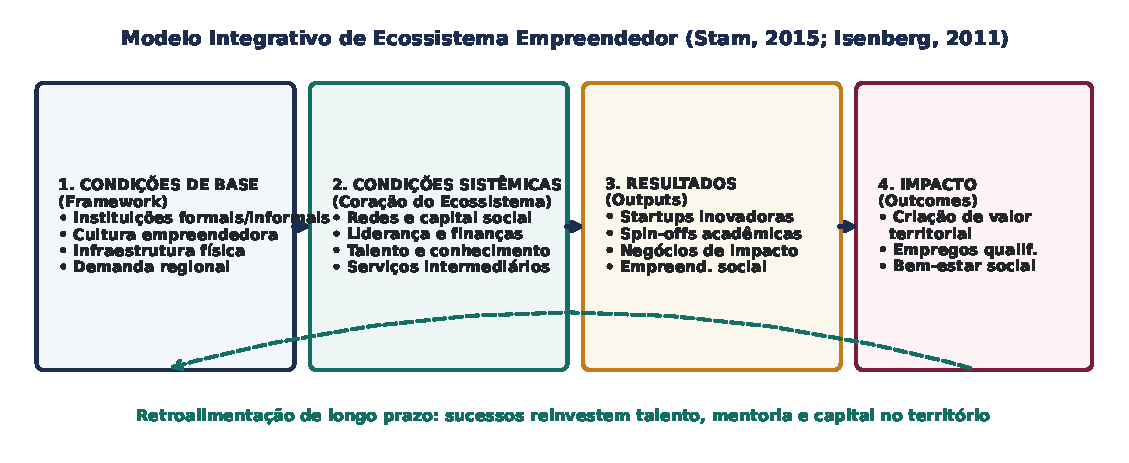
\includegraphics[width=0.94\textwidth]{figures/fig03_ecossistema_stam.pdf}
  \caption{Arquitetura multinível do Ecossistema Empreendedor segundo Stam \& van de Ven (2021) articulada aos seis domínios de Isenberg e às cinco dimensões da proximidade de Boschma (2005).}
  \label{fig:ecossistema_stam}
\end{figure}

\etapa{4}{Estudos de Caso e Aplicações Passo a Passo}

\begin{boxExemplo}{1}{Diagnóstico dos 6 Domínios de Isenberg e Efeito Gargalo}
\passoEnunciado{Uma equipe técnica avaliou os seis domínios de Isenberg em um polo regional do interior baiano (escala de $1{,}0$ a $10{,}0$), obtendo as seguintes notas: Capital Humano ($x_1 = 8{,}0$), Suporte/Universidades ($x_2 = 7{,}5$), Política ($x_3 = 6{,}0$), Cultura ($x_4 = 5{,}5$), Mercados ($x_5 = 5{,}0$) e Finanças/Capital de Risco ($x_6 = 1{,}5$).}
\passoDados{$x = (8{,}0;\; 7{,}5;\; 6{,}0;\; 5{,}5;\; 5{,}0;\; 1{,}5)$, com $n = 6$ domínios.}
\passoPedido{Calcular o índice pela média aritmética simples ($I_{\text{arit}}$) e pela média geométrica ($I_{\text{EE}}^{\text{geom}}$), explicando a diferença conceitual entre os resultados.}
\passoMetodo{Cálculo de $I_{\text{arit}} = \frac{1}{n}\sum x_i$ e $I_{\text{EE}}^{\text{geom}} = \left(\prod x_i\right)^{1/6}$.}
\passoContas{
  \begin{enumerate}[leftmargin=1.4em, itemsep=2pt]
    \item Média aritmética simples:
    \[
    I_{\text{arit}} = \frac{8{,}0 + 7{,}5 + 6{,}0 + 5{,}5 + 5{,}0 + 1{,}5}{6} = \frac{33{,}5}{6} \approx 5{,}58
    \]
    \item Produto dos seis domínios:
    \[
    \prod_{i=1}^{6} x_i = 8{,}0 \times 7{,}5 \times 6{,}0 \times 5{,}5 \times 5{,}0 \times 1{,}5
    \]
    \[
    8{,}0 \times 7{,}5 = 60{,}0; \quad 60{,}0 \times 6{,}0 = 360{,}0; \quad 360{,}0 \times 5{,}5 = 1.980{,}0; \quad 1.980{,}0 \times 5{,}0 = 9.900{,}0; \quad 9.900{,}0 \times 1{,}5 = 14.850{,}0
    \]
    \item Média geométrica (raiz sexta):
    \[
    I_{\text{EE}}^{\text{geom}} = (14.850{,}0)^{1/6} \approx 4{,}96
    \]
  \end{enumerate}
}
\passoResposta{$I_{\text{arit}} = 5{,}58$ e $I_{\text{EE}}^{\text{geom}} = 4{,}96$.}
\passoVerificacao{A média aritmética mascara a gravidade do gargalo financeiro ($1{,}5$), sugerindo um ecossistema mediano ($5{,}58$). A média geométrica penaliza o desequilíbrio ($4{,}96$). Se o território elevar Finanças de $1{,}5$ para $4{,}5$ (via fundos regionais ou subvenção), o produto triplica para $44.550$ e $I_{\text{EE}}^{\text{geom}}$ salta para $(44.550)^{1/6} \approx 5{,}95$, um ganho de quase $20\%$ no desempenho global atuando em um único gargalo.}
\end{boxExemplo}

\begin{boxExemplo}{2}{Modelo Integrativo de Stam \& van de Ven: Base vs. Sistêmicas}
\passoEnunciado{Na avaliação de dois municípios vizinhos (Município A e Município B) segundo o modelo de Stam \& van de Ven (2021), as médias das Condições de Base ($I_{\text{CB}}$) e das Condições Sistêmicas ($I_{\text{CS}}$), ambas em escala $0$--$10$, foram: Município A ($I_{\text{CB}} = 7{,}0$, $I_{\text{CS}} = 6{,}0$); Município B ($I_{\text{CB}} = 7{,}0$, $I_{\text{CS}} = 2{,}5$). Estima-se empiricamente que a taxa de \textit{output} empreendedor produtivo (EBTs por $100$ mil habitantes) siga a relação multiplicativa $O_{\text{EBT}} = 0{,}45 \times I_{\text{CB}} \times I_{\text{CS}}$.}
\passoDados{Município A: $I_{\text{CB},A} = 7{,}0$, $I_{\text{CS},A} = 6{,}0$. Município B: $I_{\text{CB},B} = 7{,}0$, $I_{\text{CS},B} = 2{,}5$. Coeficiente $k = 0{,}45$.}
\passoPedido{Calcular o \textit{output} esperado $O_{\text{EBT}}$ de cada município e a razão de desempenho entre A e B.}
\passoMetodo{Substituição direta na função de produção do ecossistema $O_{\text{EBT}} = 0{,}45 \times I_{\text{CB}} \times I_{\text{CS}}$.}
\passoContas{
  \begin{enumerate}[leftmargin=1.4em, itemsep=2pt]
    \item \textit{Output} do Município A:
    \[
    O_{\text{EBT},A} = 0{,}45 \times 7{,}0 \times 6{,}0 = 0{,}45 \times 42{,}0 = 18{,}90\text{ EBTs / 100 mil hab.}
    \]
    \item \textit{Output} do Município B:
    \[
    O_{\text{EBT},B} = 0{,}45 \times 7{,}0 \times 2{,}5 = 0{,}45 \times 17{,}5 = 7{,}875\text{ EBTs / 100 mil hab.}
    \]
    \item Razão de desempenho:
    \[
    \frac{O_{\text{EBT},A}}{O_{\text{EBT},B}} = \frac{18{,}90}{7{,}875} = 2{,}40\text{ vezes}
    \]
  \end{enumerate}
}
\passoResposta{$O_{\text{EBT},A} = 18{,}90$ e $O_{\text{EBT},B} = 7{,}875$ EBTs/$100$ mil hab. (Município A gera $2{,}40$ vezes mais EBTs).}
\passoVerificacao{Mesmo com condições de base idênticas ($I_{\text{CB}} = 7{,}0$, boa infraestrutura e segurança jurídica), a ausência de redes, liderança empreendedora e capital semente ($I_{\text{CS}} = 2{,}5$) reduz o resultado de B a menos da metade. Condições de base são necessárias, mas insuficientes sem ativação sistêmica.}
\end{boxExemplo}

\begin{boxExemplo}{3}{Ponto Ótimo da Proximidade Cognitiva (Boschma, 2005)}
\passoEnunciado{Em um programa de cooperação entre grupos de pesquisa universitários e pequenas indústrias de alimentos regionais, o desempenho inovador colaborativo ($P$, em índice de $0$ a $100$) em função da distância cognitiva $\Delta c \in [0, 10]$ é modelado pela curva em U invertido $P(\Delta c) = 24\,\Delta c - 3\,(\Delta c)^2$.}
\passoDados{$P(\Delta c) = 24\,\Delta c - 3\,(\Delta c)^2$, onde $\alpha = 24$ e $\beta = 3$.}
\passoPedido{Determinar a distância cognitiva ótima ($\Delta c^*$), o desempenho máximo $P(\Delta c^*)$ e comparar com dois casos extremos: excesso de proximidade ($\Delta c = 1$) e excesso de distância ($\Delta c = 7$).}
\passoMetodo{Derivação de $P(\Delta c)$ em relação a $\Delta c$ e igualação a zero ($\frac{dP}{d\Delta c} = 0$), seguida de avaliação pontual.}
\passoContas{
  \begin{enumerate}[leftmargin=1.4em, itemsep=2pt]
    \item Cálculo do ponto ótimo:
    \[
    \frac{dP}{d\Delta c} = 24 - 6\,\Delta c = 0 \implies 6\,\Delta c^* = 24 \implies \Delta c^* = 4{,}0
    \]
    \item Desempenho máximo em $\Delta c^* = 4{,}0$:
    \[
    P(4{,}0) = 24(4{,}0) - 3(4{,}0)^2 = 96 - 3(16) = 96 - 48 = 48{,}0
    \]
    \item Caso de excesso de proximidade ($\Delta c = 1{,}0$ — todos pensam igual):
    \[
    P(1{,}0) = 24(1{,}0) - 3(1{,}0)^2 = 24 - 3 = 21{,}0
    \]
    \item Caso de excesso de distância ($\Delta c = 7{,}0$ — falta linguagem comum):
    \[
    P(7{,}0) = 24(7{,}0) - 3(7{,}0)^2 = 168 - 3(49) = 168 - 147 = 21{,}0
    \]
  \end{enumerate}
}
\passoResposta{$\Delta c^* = 4{,}0$, com desempenho máximo $P(4{,}0) = 48{,}0$. Nos extremos ($\Delta c = 1$ ou $\Delta c = 7$), o desempenho cai para $21{,}0$ (redução de $56{,}25\%$).}
\passoVerificacao{O resultado comprova a tese de Boschma: nem a proximidade cognitiva absoluta ($\Delta c \to 0$, onde nada de novo se aprende), nem a distância extrema ($\Delta c \to 8$, onde cessa a comunicação) maximizam a inovação. A atuação de intermediários tecnológicos (NITs, consultores de extensão) serve justamente para calibrar $\Delta c$ próximo ao ponto ótimo.}
\end{boxExemplo}

\begin{boxExemplo}{4}{Paradoxo da Proximidade e Diagnóstico de \textit{Lock-in} em Rede Local}
\passoEnunciado{Uma incubadora territorial acompanha $20$ empresas de base tecnológica. Levantamento de redes mostrou que $16$ dessas empresas realizam $90\%$ de suas parcerias técnicas apenas com outras empresas da mesma cidade e ex-colegas da mesma graduação (alta proximidade social, geográfica e cognitiva), registrando taxa média de lançamento de novos produtos de $6\%$ ao ano. As outras $4$ empresas mantêm conexões híbridas com clientes e centros de pesquisa de outras regiões (proximidade balanceada), registrando taxa de $21\%$ ao ano.}
\passoDados{Grupo Fechado: $n_1 = 16$, taxa $= 6\%$/ano. Grupo Híbrido: $n_2 = 4$, taxa $= 21\%$/ano.}
\passoPedido{Calcular a taxa média ponderada de inovação do ecossistema atual e projetar a nova taxa caso políticas de conexão externa (missões técnicas e editais em rede) convertam metade do grupo fechado ($8$ empresas) para o perfil híbrido.}
\passoMetodo{Média ponderada $\bar{T} = \frac{n_1 t_1 + n_2 t_2}{n_1 + n_2}$.}
\passoContas{
  \begin{enumerate}[leftmargin=1.4em, itemsep=2pt]
    \item Taxa média atual ($n_1 = 16$, $n_2 = 4$):
    \[
    \bar{T}_{\text{atual}} = \frac{(16 \times 6\%) + (4 \times 21\%)}{20} = \frac{96\% + 84\%}{20} = \frac{180\%}{20} = 9{,}0\%\text{ ao ano}
    \]
    \item Taxa média após conversão de $8$ empresas ($n_1' = 8$, $n_2' = 12$):
    \[
    \bar{T}_{\text{proj}} = \frac{(8 \times 6\%) + (12 \times 21\%)}{20} = \frac{48\% + 252\%}{20} = \frac{300\%}{20} = 15{,}0\%\text{ ao ano}
    \]
    \item Ganho relativo sobre a taxa inicial:
    \[
    \Delta_{\text{rel}} = \frac{15{,}0 - 9{,}0}{9{,}0} \times 100\% = 66{,}67\%
    \]
  \end{enumerate}
}
\passoResposta{A taxa média do ecossistema sobe de $9{,}0\%$ para $15{,}0\%$ ao ano (aumento relativo de $66{,}67\%$).}
\passoVerificacao{O exercício quantifica o paradoxo da proximidade de Boschma: excesso de confiança fechada e homofilia acadêmica gera redundância informacional. Abrir ``pontes externas'' sem destruir o enraizamento local rompe o \textit{lock-in} cognitivo.}
\end{boxExemplo}

\begin{boxExemplo}{5}{Contraponto às \textit{Gazelles}: Retenção Territorial de Emprego e Renda}
\passoEnunciado{Um fundo estadual dispõe de $\reais{3.000.000}$ em fomento e analisa duas carteiras alternativas para $5$ anos: (A) apostar integralmente em $1$ startup \textit{gazelle} de plataforma digital urbana que gera $25$ empregos locais altamente remunerados ($\reais{8.000}$/mês médios), mas terceiriza $70\%$ de sua operação em nuvem internacional e planeja transferir a sede após a rodada Série A no ano $3$; (B) apoiar $10$ PMEs tecnológicas territoriais ($\reais{300.000}$ cada) em bioeconomia e automação regional que geram $8$ empregos diretos cada ($\reais{4.500}$/mês médios), permanecendo enraizadas pelos $5$ anos completos.}
\passoDados{Orçamento $= \reais{3.000.000}$; horizonte $= 60$ meses ($5$ anos); Opção A: $25$ empregos por $36$ meses a $\reais{8.000}$/mês; Opção B: $10 \times 8 = 80$ empregos por $60$ meses a $\reais{4.500}$/mês.}
\passoPedido{Calcular a massa salarial acumulada retida no território em cada opção ao longo dos $5$ anos e o custo público por emprego-ano gerado.}
\passoMetodo{Massa salarial $= N_{\text{emp}} \times W_{\text{mês}} \times M_{\text{meses}}$. Empregos-ano $= N_{\text{emp}} \times (\text{anos de permanência})$.}
\passoContas{
  \begin{enumerate}[leftmargin=1.4em, itemsep=2pt]
    \item Opção A (\textit{Gazelle}, $3$ anos $= 36$ meses no território):
    \[
    \text{Massa}_A = 25 \times 8.000 \times 36 = \reais{7.200.000}
    \]
    \[
    \text{Empregos-ano}_A = 25 \times 3 = 75\text{ empregos-ano} \implies \text{Custo} = \frac{3.000.000}{75} = \reais{40.000}\text{/emprego-ano}
    \]
    \item Opção B ($10$ PMEs enraizadas, $5$ anos $= 60$ meses):
    \[
    \text{Massa}_B = 80 \times 4.500 \times 60 = \reais{21.600.000}
    \]
    \[
    \text{Empregos-ano}_B = 80 \times 5 = 400\text{ empregos-ano} \implies \text{Custo} = \frac{3.000.000}{400} = \reais{7.500}\text{/emprego-ano}
    \]
  \end{enumerate}
}
\passoResposta{A Opção B retém $\reais{21.600.000}$ em massa salarial ($3{,}0$ vezes mais que a Opção A) a um custo de $\reais{7.500}$ por emprego-ano (contra $\reais{40.000}$ na Opção A).}
\passoVerificacao{Sem negar o papel das empresas de alto crescimento, os números expõem o risco de políticas periféricas focadas exclusivamente em \textit{gazelles} móveis: quando o capital e a sede migram após rodadas externas, o território subsidia a etapa de maior risco e perde os \textit{outcomes} de longo prazo.}
\end{boxExemplo}

\etapa{5}{Armadilhas Conceituais e Erros Mais Comuns}

\begin{boxErro}[Erro 1: Confundir Sistema Regional de Inovação (SRI) com Ecossistema Empreendedor (EE)]
Embora ambos tratem da dimensão territorial da inovação, o SRI coloca foco nas instituições de P\&D, universidades e firmas incumbentes, enquanto o EE coloca o empreendedor como agente central da criação de novos negócios. Tratar um parque tecnológico universitário sem empreendedores ativos como um EE maduro confunde infraestrutura acadêmica com dinamismo empreendedor.
\end{boxErro}

\begin{boxErro}[Erro 2: Usar Média Aritmética para Mascarar Gargalos Sistêmicos]
Em diagnósticos de ecossistemas (Isenberg e Stam), compensar uma nota péssima em Finanças ou Mercados com notas altas em Universidades via média aritmética esconde a trava estrutural do sistema. Um ecossistema funciona como cadeia multiplicativa: sem capital ou compradores iniciais, a pesquisa acadêmica não se converte em negócios sustentáveis.
\end{boxErro}

\begin{boxErro}[Erro 3: Assumir que ``Mais Proximidade'' é Sempre Melhor]
Um equívoco frequente em projetos de incubadoras e redes locais é supor que aproximar indefinidamente os atores maximiza a inovação. Como demonstrou Boschma (2005), proximidade cognitiva ou social excessiva gera redundância e \textit{lock-in}, exigindo abertura controlada a conhecimentos e parceiros externos.
\end{boxErro}

\begin{boxErro}[Erro 4: Importar Modelos de \textit{Gazelles} sem Leitura de Retenção Local]
Copiar métricas do Vale do Silício (número de unicórnios e rodadas de \textit{venture capital}) em regiões com baixa densidade financeira e cadeias agroindustriais tradicionais induz políticas que ignoram oportunidades reais de inovação incremental, bioeconomia e PMEs tecnológicas enraizadas.
\end{boxErro}

\etapa{6}{Lista de Exercícios (15 Questões Graduadas)}

\subsection*{Bloco A — Conceituais e Básicos (Questões 1 a 5)}

\begin{enumerate}[leftmargin=1.6em, itemsep=6pt]
  \item Explique a diferença central entre a abordagem dos Sistemas Regionais de Inovação (SRI) e a dos Ecossistemas Empreendedores (EE) quanto ao protagonista do processo inovativo.
  \espacoResolucao[1.8cm]

  \item Liste os seis domínios do Ecossistema Empreendedor de Daniel Isenberg (2011) e indique dois elementos concretos que compõem o domínio de \textit{Suporte}.
  \espacoResolucao[1.8cm]

  \item No modelo de Stam \& van de Ven (2021), diferencie \textit{condições de base}, \textit{condições sistêmicas}, \textit{outputs} e \textit{outcomes}.
  \espacoResolucao[1.8cm]

  \item Um ecossistema regional obteve notas $9{,}0$, $9{,}0$, $9{,}0$ e $1{,}0$ em quatro pilares analisados. Calcule a média aritmética e a média geométrica dessas notas e comente o efeito do pilar mais fraco.
  \espacoResolucao[1.8cm]

  \item Defina brevemente cada uma das cinco dimensões da proximidade propostas por Ron Boschma (2005).
  \espacoResolucao[1.8cm]
\end{enumerate}

\subsection*{Bloco B — Intermediários e Aplicados (Questões 6 a 10)}

\begin{enumerate}[leftmargin=1.6em, itemsep=6pt, resume]
  \item Em um diagnóstico territorial baseado em Stam \& van de Ven (2021), as Condições de Base receberam escore $I_{\text{CB}} = 8{,}0$ e as Condições Sistêmicas receberam $I_{\text{CS}} = 3{,}0$. Utilizando $O_{\text{EBT}} = 0{,}50 \times I_{\text{CB}} \times I_{\text{CS}}$, calcule o \textit{output} atual e o novo \textit{output} caso uma política de redes e capital semente eleve $I_{\text{CS}}$ para $5{,}5$.
  \espacoResolucao[2.2cm]

  \item Considere que o desempenho inovador de parcerias entre EBTs e cooperativas agrícolas siga a função $P(\Delta c) = 30\,\Delta c - 2{,}5\,(\Delta c)^2$, onde $\Delta c$ é a distância cognitiva ($0$ a $10$). Calcule a distância cognitiva ótima ($\Delta c^*$) e o desempenho máximo $P(\Delta c^*)$.
  \espacoResolucao[2.2cm]

  \item Explique como o excesso de proximidade social e institucional pode gerar \textit{lock-in} cognitivo em um polo tecnológico regional e proponha duas ações práticas para mitigar esse paradoxo.
  \espacoResolucao[2.0cm]

  \item Avalie criticamente a priorização exclusiva de empresas \textit{gazelles} em editais públicos estaduais no Nordeste brasileiro frente ao desenvolvimento territorial de médio e longo prazo.
  \espacoResolucao[2.0cm]

  \item Um município do interior apresenta forte proximidade geográfica e social entre suas empresas, mas baixa proximidade cognitiva com a universidade local ($\Delta c = 9{,}0$). Como a criação de um Núcleo de Inovação Tecnológica (NIT) ou escritório de extensão pode atuar sobre as dimensões de Boschma?
  \espacoResolucao[2.0cm]
\end{enumerate}

\subsection*{Bloco C — Questões Objetivas de Fixação (Questões 11 a 15)}

\begin{enumerate}[leftmargin=1.6em, itemsep=6pt, resume]
  \item No modelo de Ecossistema Empreendedor de Daniel Isenberg (2011), a tolerância ao fracasso honesto, a visibilidade de empreendedores locais e a aceitação social do risco pertencem ao domínio:
  \begin{alternativas}
    \item Política.
    \item Finanças.
    \item Cultura.
    \item Suporte.
    \item Mercados.
  \end{alternativas}

  \item No modelo integrativo de Stam (2015) e Stam \& van de Ven (2021), representam respectivamente uma \textbf{condição de base}, uma \textbf{condição sistêmica} e um \textbf{\textit{outcome}}:
  \begin{alternativas}
    \item Redes de mentoria, criação de startups e infraestrutura rodoviária.
    \item Instituições formais/segurança jurídica, financiamento/talento especializado e geração de valor agregado/bem-estar territorial.
    \item Capital de risco, cultura empreendedora e número de patentes depositadas.
    \item Demanda agregada, infraestrutura física e política monetária nacional.
    \item Serviços jurídicos, instituições formais e existência de parques tecnológicos.
  \end{alternativas}

  \item Segundo Ron Boschma (2005), a dimensão da proximidade que se refere ao grau em que dois atores compartilham bases de conhecimento e linguagem técnica suficientes para absorver e processar novas informações é a proximidade:
  \begin{alternativas}
    \item Geográfica.
    \item Social.
    \item Institucional.
    \item Cognitiva.
    \item Organizacional.
  \end{alternativas}

  \item Sobre o paradoxo da proximidade formulado por Boschma (2005), é correto afirmar que:
  \begin{alternativas}
    \item A distância cognitiva nula ($\Delta c = 0$) garante o maior volume possível de inovações radicais.
    \item A proximidade geográfica substitui integralmente todas as demais dimensões de proximidade.
    \item Tanto a ausência quanto o excesso de proximidade podem prejudicar a inovação, gerando falta de coordenação no primeiro caso e \textit{lock-in} no segundo.
    \item Redes sociais altamente fechadas impedem qualquer risco de acomodação ou redundância informacional.
    \item A proximidade institucional impede o surgimento de conflitos regulatórios ou de normas informais.
  \end{alternativas}

  \item Se quatro domínios de um ecossistema apresentam escores $4{,}0$, $4{,}0$, $9{,}0$ e $9{,}0$, sua média geométrica $I_{\text{EE}}^{\text{geom}}$ é exatamente igual a:
  \begin{alternativas}
    \item $5{,}5$
    \item $6{,}0$
    \item $6{,}5$
    \item $7{,}0$
    \item $7{,}5$
  \end{alternativas}
\end{enumerate}

\etapa{7}{Questões de Alta Complexidade (Estilo ANPAD / Pós-Graduação / CT\&I)}

\begin{enumerate}[leftmargin=1.6em, itemsep=8pt]
  \item \textbf{(Estilo Pós-Graduação / Desenvolvimento Territorial)} Considere as afirmações sobre Ecossistemas Empreendedores e Proximidades:
  \begin{itemize}[leftmargin=1.2em, itemsep=2pt]
    \item[I.] A existência de proximidade organizacional ou cognitiva forte permite que colaborações inovadoras ocorram mesmo entre atores geograficamente distantes, mostrando que a proximidade física não é condição absoluta.
    \item[II.] No modelo de Stam \& van de Ven (2021), as condições de base determinam isoladamente o surgimento de empresas de alto impacto, dispensando a formação de redes empreendedoras locais.
    \item[III.] Políticas de fomento voltadas exclusivamente a \textit{gazelles} podem subestimar o potencial multiplicador de PMEs tecnológicas enraizadas em cadeias produtivas regionais.
  \end{itemize}
  Está correto o que se afirma em:
  \begin{alternativas}
    \item I, apenas.
    \item II, apenas.
    \item I e III, apenas.
    \item II e III, apenas.
    \item I, II e III.
  \end{alternativas}

  \item \textbf{(Estilo ANPAD / Modelagem de Ecossistemas)} Um pesquisador modelou o desempenho colaborativo entre universidades e empresas em dois setores territoriais: no Setor Alfa, $P_A(\Delta c) = 18\,\Delta c - 1{,}5\,(\Delta c)^2$; no Setor Beta, $P_B(\Delta c) = 20\,\Delta c - 2{,}5\,(\Delta c)^2$. Comparando os pontos ótimos de distância cognitiva ($\Delta c^*$) e os respectivos desempenhos máximos ($P_{\max}$), conclui-se que:
  \begin{alternativas}
    \item $\Delta c_A^* = 6{,}0$ com $P_{A,\max} = 54{,}0$; $\Delta c_B^* = 4{,}0$ com $P_{B,\max} = 40{,}0$.
    \item $\Delta c_A^* = 4{,}0$ com $P_{A,\max} = 40{,}0$; $\Delta c_B^* = 6{,}0$ com $P_{B,\max} = 54{,}0$.
    \item $\Delta c_A^* = 12{,}0$ com $P_{A,\max} = 108{,}0$; $\Delta c_B^* = 8{,}0$ com $P_{B,\max} = 80{,}0$.
    \item Ambos possuem o mesmo ponto ótimo $\Delta c^* = 5{,}0$, variando apenas o nível máximo de desempenho.
    \item O Setor Beta apresenta maior desempenho máximo por tolerar maior distância cognitiva.
  \end{alternativas}

  \item \textbf{(Estilo Concurso CT\&I / Políticas de Inovação)} Um estado brasileiro investiu pesadamente na construção de prédios de parques tecnológicos (infraestrutura física) e na reforma de leis estaduais de desburocratização, mas após cinco anos registrou baixíssima taxa de criação de EBTs e saída precoce de startups para São Paulo. À luz de Isenberg (2011) e Stam (2015), a explicação mais precisa para esse resultado é:
  \begin{alternativas}
    \item A criação de infraestrutura física e legal (condições de base) é suficiente para gerar \textit{outputs}, indicando erro na mensuração estatística.
    \item A política concentrou-se em condições de base e infraestrutura sem ativar condições sistêmicas críticas como capital semente local, redes de mentoria empreendedora e mercados compradores regionais.
    \item O modelo de Isenberg recomenda eliminar as universidades do ecossistema para acelerar o surgimento de empresas.
    \item A saída de startups comprova que a proximidade institucional impede qualquer vínculo com investidores externos.
    \item O problema decorre exclusivamente do excesso de proximidade cognitiva entre os prédios do parque tecnológico.
  \end{alternativas}
\end{enumerate}

\begin{boxDica}[Contraponto Crítico e Prática Territorial (Conexão AV1 e AV3)]
Na \textbf{AV1}, ao comparar um ecossistema periférico com um polo metropolitano usando Isenberg ou Stam, evite diagnósticos genéricos do tipo ``falta apoio''. Identifique exatamente qual condição sistêmica (finanças, redes, mercados âncora) está agindo como gargalo multiplicativo. Na \textbf{AV3}, demonstre como seu empreendimento ou política utiliza as cinco proximidades de Boschma para conectar o saber acadêmico ao setor produtivo local sem cair em redes fechadas.
\end{boxDica}

\clearpage
\etapa{8}{Gabarito Comentado (Questões 1 a 18)}

\begin{boxGabarito}[Respostas Comentadas — Exercícios 1 a 15 e Questões de Alta Complexidade 16 a 18]
\begin{enumerate}[leftmargin=1.6em, itemsep=4pt]
  \item \textbf{Resposta:} O SRI foca na arquitetura institucional de geração e difusão de conhecimento (universidades, ICTs, políticas de P\&D e firmas estabelecidas), enquanto o EE coloca o empreendedor ambicioso como agente central, analisando como recursos e redes se articulam para criar e escalar negócios.
  \item \textbf{Resposta:} Os seis domínios de Isenberg são: Política, Finanças, Cultura, Suporte, Capital Humano e Mercados. Exemplos em \textit{Suporte}: infraestrutura física/digital (incubadoras, banda larga) e serviços especializados (contabilidade, advogados de PI).
  \item \textbf{Resposta:} Condições de base são os fundamentos estruturais (instituições, cultura, infraestrutura, demanda); condições sistêmicas são o motor ativo do ecossistema (redes, liderança, finanças, talento, conhecimento, intermediários); \textit{outputs} são as realizações empreendedoras (novas EBTs/inovações); \textit{outcomes} são os resultados finais de desenvolvimento (valor agregado, empregos e bem-estar territorial).
  \item \textbf{Resposta:} Média aritmética $= (9+9+9+1)/4 = 28/4 = 7{,}00$. Média geométrica $= (9 \times 9 \times 9 \times 1)^{1/4} = (729)^{1/4} = 27^{1/2} \approx 5{,}20$. A média geométrica reflete o efeito gargalo do pilar com nota $1{,}0$.
  \item \textbf{Resposta:} Geográfica (distância física); Cognitiva (base de conhecimento compartilhada); Organizacional (coordenação em arranjos formais/redes); Social (confiança e laços interpessoais); Institucional (normas formais e informais comuns).
  \item \textbf{Resposta:} Atual: $O_1 = 0{,}50 \times 8{,}0 \times 3{,}0 = 12{,}0$ EBTs/$100$ mil hab. Novo: $O_2 = 0{,}50 \times 8{,}0 \times 5{,}5 = 22{,}0$ EBTs/$100$ mil hab. (incremento de $83{,}3\%$).
  \item \textbf{Resposta:} $\frac{dP}{d\Delta c} = 30 - 5\,\Delta c = 0 \implies \Delta c^* = 6{,}0$. Desempenho máximo: $P(6{,}0) = 30(6) - 2{,}5(36) = 180 - 90 = 90{,}0$.
  \item \textbf{Resposta:} O excesso de proximidade social e institucional faz os atores repetirem rotinas e rejeitarem ideias externas (\textit{lock-in} cognitivo). Ações mitigadoras: editais obrigando parcerias inter-regionais e programas de intercâmbio técnico com outros ecossistemas.
  \item \textbf{Resposta:} Focar apenas em \textit{gazelles} pode drenar recursos escassos para poucos negócios que frequentemente migram de sede em busca de capital externo, enquanto PMEs tecnológicas locais geram mais empregos duradouros e retenção de renda regional.
  \item \textbf{Resposta:} O NIT atua como tradutor cognitivo e organizacional, reduzindo $\Delta c$ de $9{,}0$ para uma faixa funcional e criando pontes formais (contratos de P\&D, prestação de serviços) entre universidade e empresas locais.
  \item \textbf{Gabarito: (C).} Tolerância ao risco/fracasso e valorização do empreendedor compõem o domínio Cultura.
  \item \textbf{Gabarito: (B).} Instituições formais = condição de base; financiamento/talento = condição sistêmica; valor agregado/bem-estar = \textit{outcome}.
  \item \textbf{Gabarito: (D).} Proximidade cognitiva refere-se à base compartilhada de conhecimento e capacidade de absorção.
  \item \textbf{Gabarito: (C).} Tanto a distância excessiva quanto a proximidade excessiva prejudicam o desempenho inovador (curva em U invertido).
  \item \textbf{Gabarito: (B).} $(4 \times 4 \times 9 \times 9)^{1/4} = (16 \times 81)^{1/4} = 2 \times 3 = 6{,}0$.
  \item \textbf{Gabarito: (C).} A assertiva II é falsa pois condições de base precisam ser ativadas pelas condições sistêmicas.
  \item \textbf{Gabarito: (A).} Setor Alfa: $18 - 3\,\Delta c = 0 \implies \Delta c_A^* = 6{,}0$, $P_A(6) = 18(6) - 1{,}5(36) = 108 - 54 = 54{,}0$. Setor Beta: $20 - 5\,\Delta c = 0 \implies \Delta c_B^* = 4{,}0$, $P_B(4) = 20(4) - 2{,}5(16) = 80 - 40 = 40{,}0$.
  \item \textbf{Gabarito: (B).} Prédios e leis são condições de base/suporte; faltaram condições sistêmicas (capital, redes, compradores locais).
\end{enumerate}
\end{boxGabarito}

\begin{boxResumo}
\begin{itemize}[leftmargin=1.4em, itemsep=2pt]
  \item SRIs enfocam instituições de conhecimento e P\&D; Ecossistemas Empreendedores enfocam o empreendedor e a articulação dinâmica de recursos.
  \item Isenberg (2011) organiza o ecossistema em 6 domínios (Política, Finanças, Cultura, Suporte, Capital Humano e Mercados).
  \item Stam \& van de Ven (2021) distinguem condições de base e sistêmicas que geram \textit{outputs} empreendedores e \textit{outcomes} territoriais, capturados de forma não compensatória pela média geométrica.
  \item Boschma (2005) define 5 proximidades e alerta para o paradoxo da proximidade (\textit{lock-in}), complementado pela crítica à obsessão por \textit{gazelles}.
\end{itemize}
\end{boxResumo}

\begin{boxTeste}
Responda sem consultar o texto e confira o gabarito logo abaixo:
\begin{enumerate}[leftmargin=1.4em, itemsep=3pt]
  \item (\V\ / \F) No modelo de Stam \& van de Ven (2021), infraestrutura física e instituições formais são classificadas como condições sistêmicas.
  \item (\V\ / \F) Na curva em U invertido de Boschma, o máximo desempenho inovador ocorre em um nível intermediário de distância cognitiva.
  \item (\V\ / \F) A média geométrica é mais sensível a gargalos em um único domínio do ecossistema do que a média aritmética.
  \item (\V\ / \F) Políticas voltadas apenas para empresas \textit{gazelles} garantem automaticamente maior retenção salarial em territórios periféricos.
\end{enumerate}
\vspace{4pt}
\textbf{Gabarito do Checkpoint:} 1. \F\ (são condições de base); 2. \V; 3. \V; 4. \F\ (há risco de migração de sede e menor retenção territorial).
\end{boxTeste}
